\section{Virtual Reality}

With the launch and success of modern technologies like Oculus Rift, HTC Vive, or Playstation VR, today’s virtual reality (VR) is mostly associated with a head-mounted device that provides this experience for the wearer. Virtual reality headsets combine a stereoscopic head-mounted display (HMD), stereophonic sound, and sensors like gyroscopes or accelerometers for head motion tracking. The main goal of these devices is to fool user’s senses, make him feel present and immersed in virtual reality. A person using such equipment is able to move and look around artificial world. The illusion of 3D depth is achieved by presenting two offset images separately to the left and right eye of the user (see Figure \ref{fig:STEREOSCOPIC}). Usually users can also interact with the virtual world's features by using specially designed controllers. Today VR headsets are mostly used for gaming, simulations, education, and other entertainment purposes.

\begin{figure}[th]
\centering
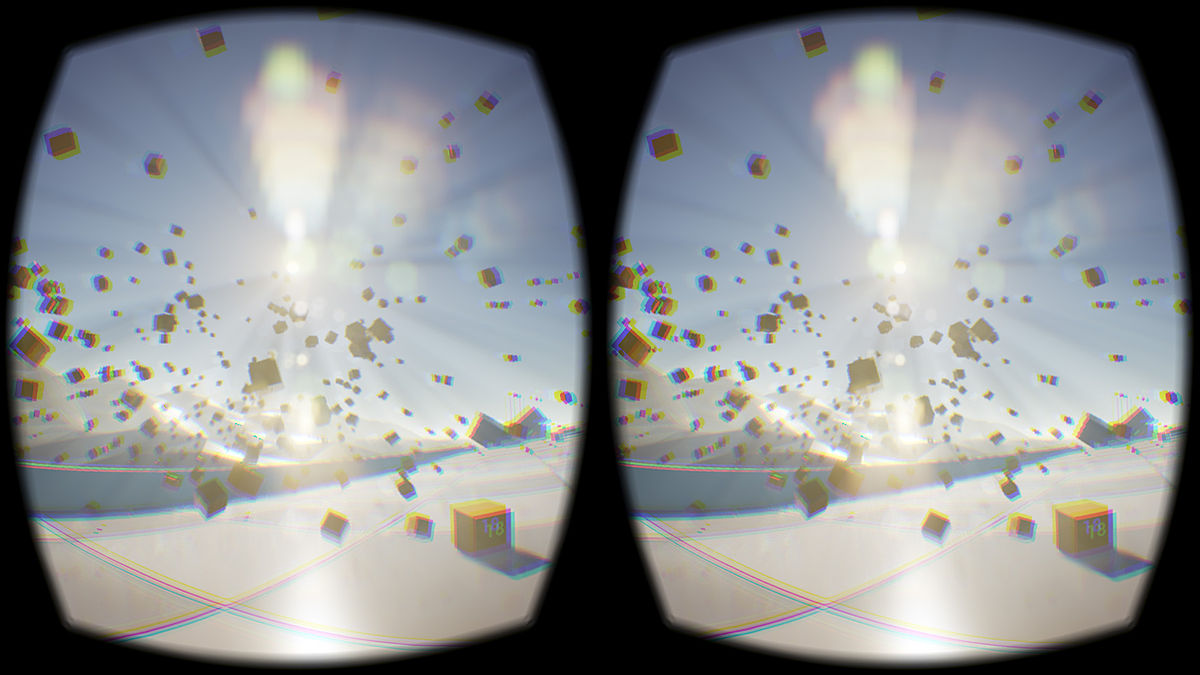
\includegraphics[width=0.85\textwidth]{img/stereoscopic.jpg}
\caption{An example of the stereoscopic image that is displayed in VR headset (image source: \cite{STEREOSCOPIC_IMAGE}).}
\label{fig:STEREOSCOPIC}
\end{figure}

The concept of virtual reality is evolving and changing quickly. The technologies we use now will probably become obsolete in next 5 years. To describe what virtual Reality really means, the definition must be broad enough to enclose what it meant in the past, what it is today, and what it can become in the future. S. M. LaValle in his book \cite{VR_BOOK} tries this approach to define VR in general way. The four key concepts that appear in his VR description are:

\begin{itemize}
\item \textit{Targeted behavior}: The experience from the real world we try to replicate. It could be anything from walking, dancing, swimming, shooting arrows, etc.
\item \textit{Organism}: Any life form can be the user of VR. In the past it was tested even on animals like cockroaches, fishes, monkeys and rodents.
\item \textit{Artificial sensory stimulation}: With the use of available equipment and technology, organism’s senses are tricked to make him feel present in artificial reality.
\item \textit{Awareness}: While being immersed in VR, the user should be oblivious to any interference. Feeling presence in this altered or another world is accepted as natural.
\end{itemize}

Virtual reality has a long history that can be traced back even to 1962, when Morton Heilig built a machine called Sensorama. The machine could provide body tilting, supply stereo sound, display stereoscopic 3-D images, and trigger tracks of aromas and wind during the film \cite{SENSORAMA}. Later in 1968, Ivan Sutherland invented what is regarded as the first head-mounted display device: The Sword of Damocles. The system provided basic user interface and realism. The graphics of created VR were simple wire-frame model rooms \cite{DAMOCLES}. The device was so heavy that it had to be attached to the ceiling with a mechanical arm (see Figure \ref{fig:FIRST_VR}). In the next years VR devices were mainly used for flight simulation, military training, medical purposes, and automobile design. With the advancements in technology and the launch of an affordable high-quality VR headsets, virtual reality became more accessible for video game players. Today we are witnessing an exciting rebirth of interest in VR, not only in entertainment industry but also in academic research.

\begin{figure}[th]
\centering
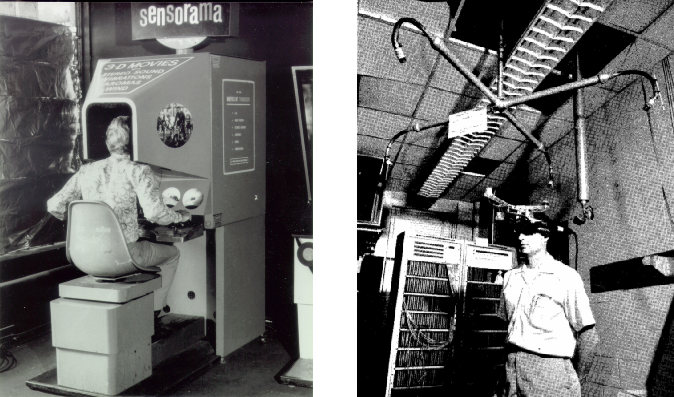
\includegraphics[width=0.85\textwidth]{img/first_vr.png}
\caption{The Sensorama and the Sword of Damocles, the first attempts at creating virtual reality (image source: \cite{SENSORAMA_IMAGE}\cite{DAMOCLES}).}
\label{fig:FIRST_VR}
\end{figure}

The renewed interest in VR started in 2012, when a Kickstarter crowdfunding campaign for Oculus Rift (see Figure \ref{fig:CONTROLLERS}) ended with a huge success. The campaign promised an affordable high-quality VR headset to the public, and it received the funding of \$250000 in less than 24 hours \cite{VR_TECHNOLOGY}. Before the final consumer version of Oculus Rift was released on 28 March 2016, the product went through many prototypes: the Development Kit 1, the Crystal Cove, the Development Kit 2, and the Crescent Bay. Over 500 applications were made during the time the two development kits were available for the researchers and campaign's backers. In the following years, other companies developed their own consumer-oriented VR headsets and tried to replicate the success of Oculus Rift. The two big competitors are the HTC Vive and the PlayStation VR. While the Oculus Rift and the PlayStation VR are mainly focused on a seated VR experience, the HTC Vive is specially designed for a room-scale VR experience that allows users to freely walk around a 5m x 5m tracked space. There are also various mobile HMDs, such as the Google Cardboard and the GearVR, that allow using a couple of selected models of smartphones for display and processing of data. The smartphone is inserted into a simple case that keeps it at a short range from the lenses. These devices offer a cheap introduction to VR experience, however, they are not equipped with advanced tracking systems, and they cannot handle more demanding games.

\begin{figure}[th]
\centering
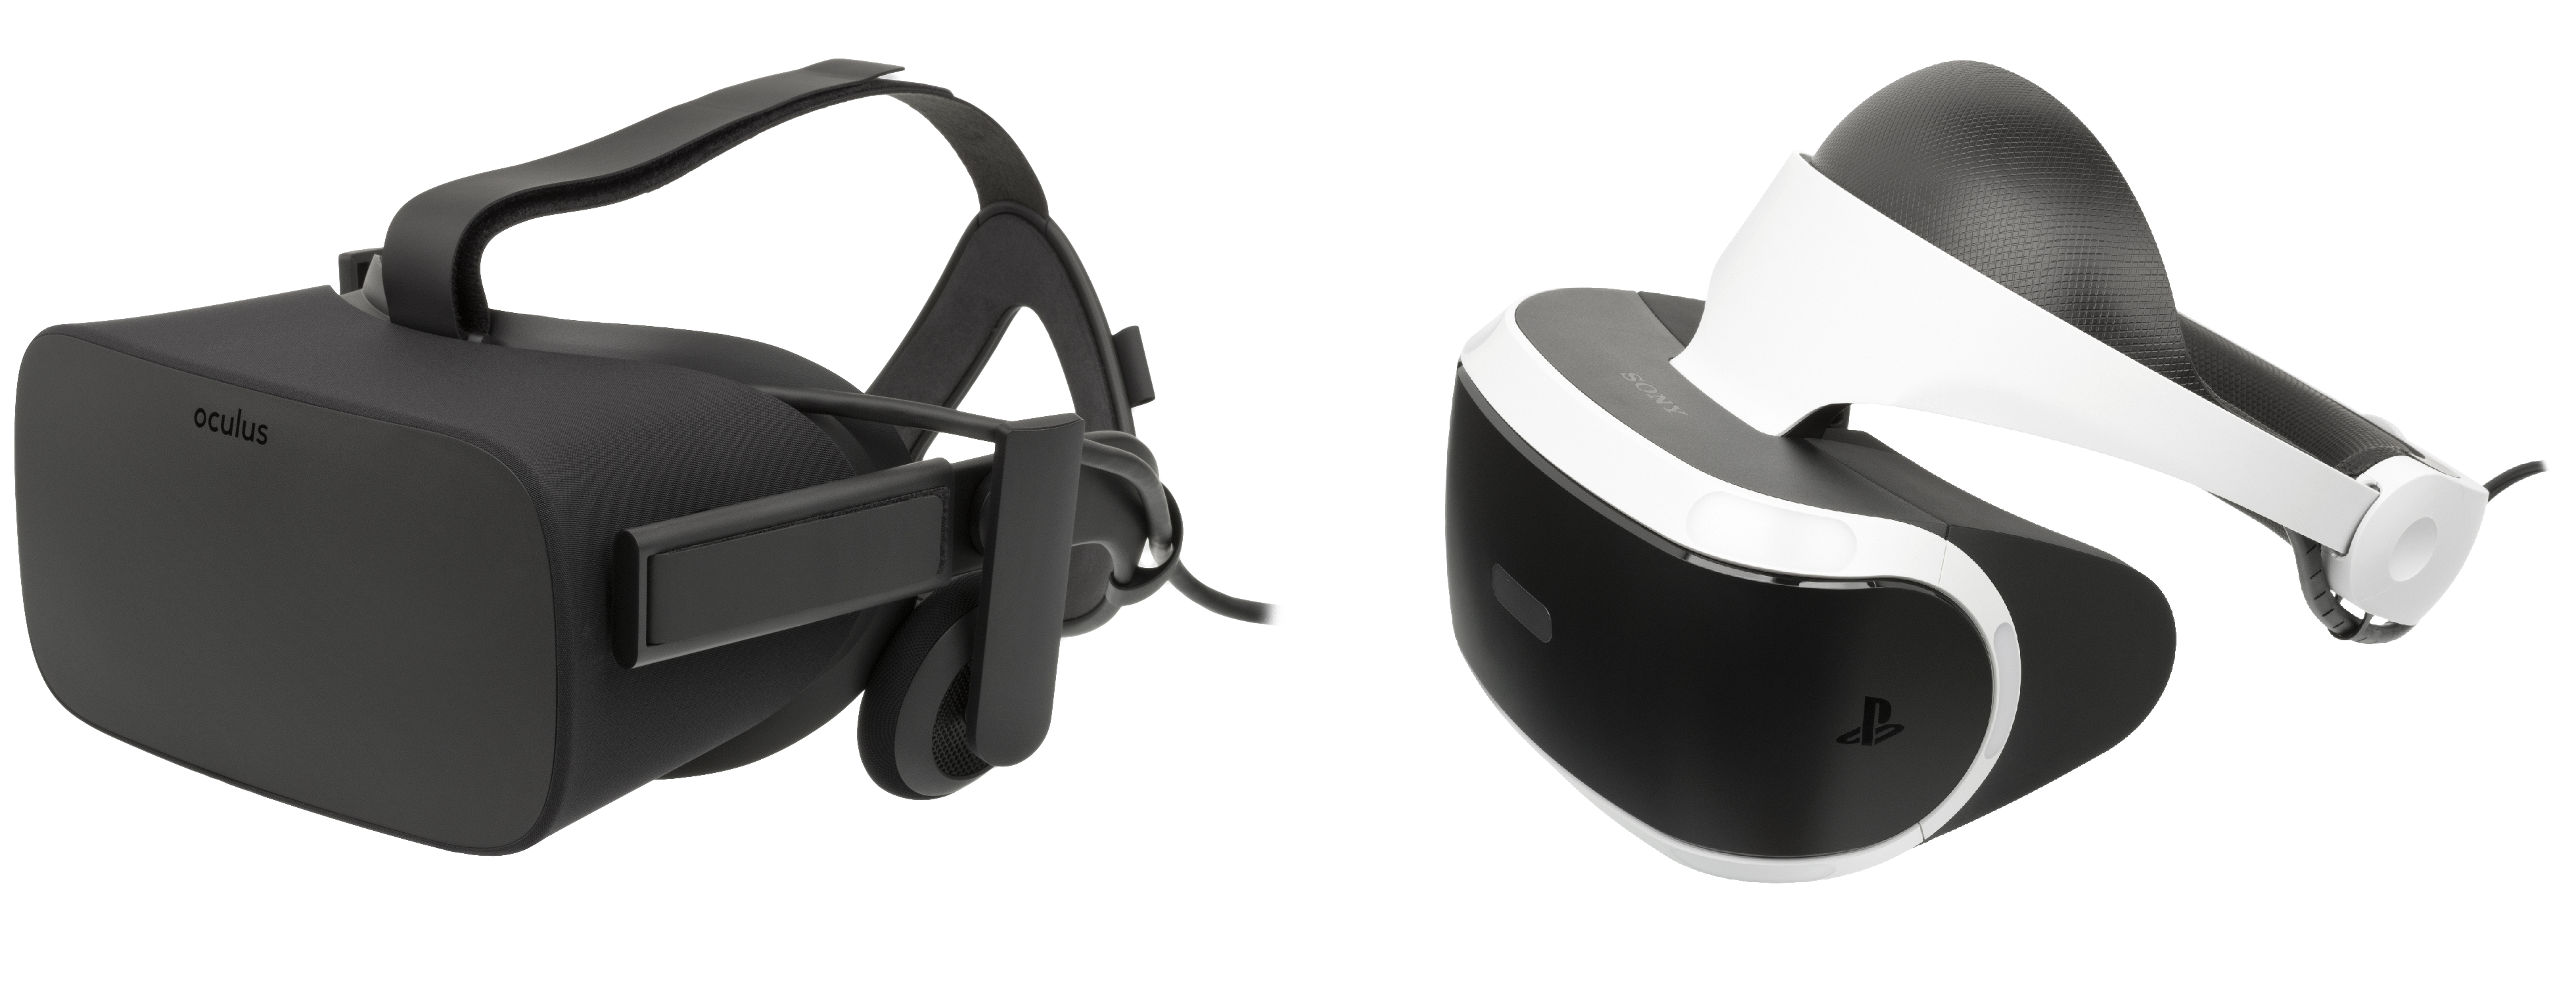
\includegraphics[width=1\textwidth]{img/headsets.png}
\caption{Modern popular VR headsets: the Oculus Rift and the Playstation VR (image source: \cite{OCULUS_HEADSET}\cite{PSVR_HEADSET}).}
\label{fig:CONTROLLERS}
\end{figure}

\section{VR Input Methods}

As more companies enter the VR headset market, we can observe a rapid technological advancement in input devices. Authors of the article \textit{State of the Art of Virtual Reality Technology} \cite{VR_TECHNOLOGY} identified three different categories for devices handling input in VR: controllers, navigation devices, and tracking technologies. Most of the controllers for VR headsets are hand worn and provide 6DoF (Six Degrees of Freedom) tracking information. They are usually equipped with buttons for discrete input, and top-mounted touchpads or joysticks for analog input. For example, Vive Controller (see Figure \ref{fig:CONTROLLERS_IMAGE}) features 24 sensors, a multi-function trackpad, and a dual-stage trigger \cite{VIVE_IMAGE}.

\begin{figure}[th]
\centering
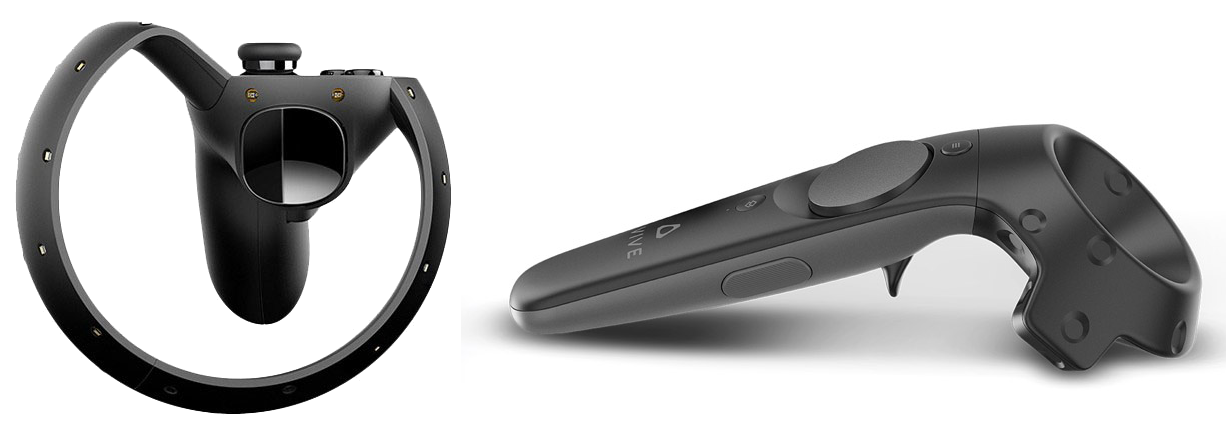
\includegraphics[width=1\textwidth]{img/modern_controllers.png}
\caption{Modern VR controllers: the Oculus Touch and the HTC Vive Controller (image source: \cite{VR_TECHNOLOGY}\cite{VIVE_IMAGE}).}
\label{fig:CONTROLLERS_IMAGE}
\end{figure}

The illusion of traversing an endless space can be achieved with the help of navigation devices. Most devices in this category work similar to traditional treadmills, permitting movement in only one direction. However, some of them allow motion on a two-dimensional plane. For example, Virtuix Omni (see Figure \ref{fig:VIRTUX_IMAGE}) is a concave platform with a low-friction surface, which allows locomotive motion in any direction. There are also attempts at creating devices less expensive and more affordable to general public. Google is currently working on motorized shoes that allow an endless movement in a limited space \cite{VR_SHOES}. Other researchers experiment with devices that were not specially designed for virtual reality. For instance, A. Aguirre in his master thesis \cite{JOYSTICK} describes the process of navigation in VR through leaning on the Wii Balance Board.

\begin{figure}[th]
\centering
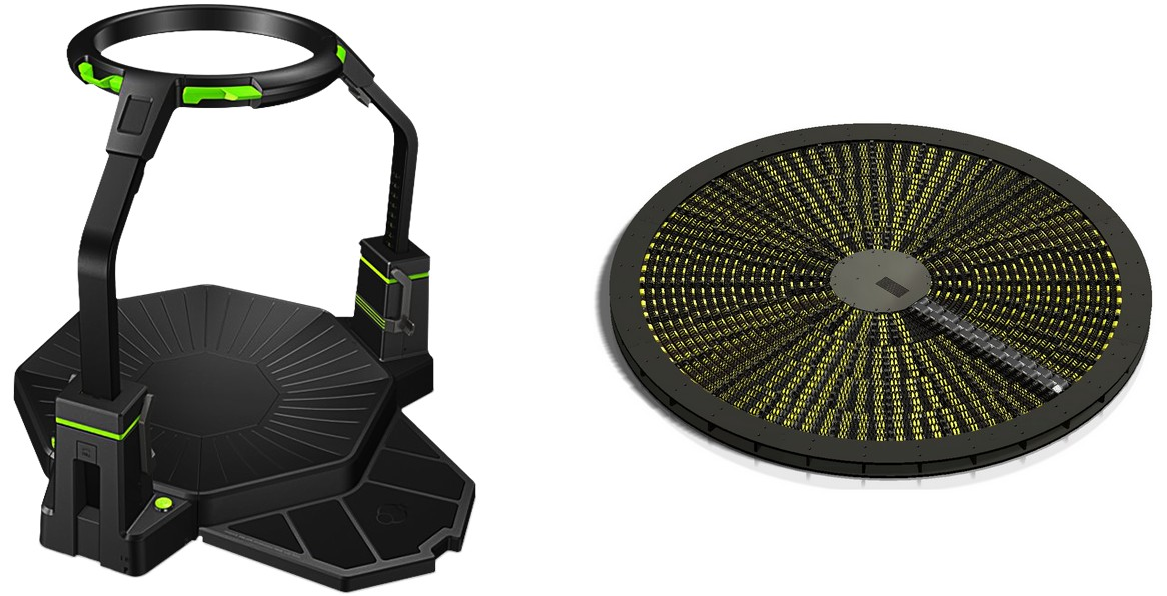
\includegraphics[width=0.85\textwidth]{img/vr_threadmills.png}
\caption{Omnidirectional treadmills: the Virtuix Omni and the WalkMouse (image source: \cite{VR_TECHNOLOGY}).}
\label{fig:VIRTUX_IMAGE}
\end{figure}

There are currently two approaches for motion tracking technologies. First is full body tracking, which focuses on posture and upper body of the users. Second is gesture tracking, which is usually achieved optically or with devices worn on hands. Full body tracking is commonly implemented using magnetic tracking or Inertial Measurement Units (IMUs), providing six degrees of freedom by placing orthogonally to each other accelerometers, gyroscopes, and magnetometers. IMUs are used to perform rotational tracking for the controllers and HMDs. They measure the rotational movements of the yaw, pitch, and roll. Valve came up with different approach, their inside-out Lighthouse tracking system involves two Base Stations that scan the tracked space with lasers \cite{VIVE}. These Base Stations (see Figure \ref{fig:BASE_STATIONS}) are small cube-shaped devices placed in opposite sides of the room. They constantly sweep the area with non-visible lights that the receptors on the HMDs and controllers intercept. The stations serve as reference points for these tracked devices, allowing them to figure out where they are in the 3D space. 

Gesture tracking can be achieved with numerous input devices that are not necessarily designed for VR. For example, the Leap Motion technology is designed to track hands and fingers with low processing power, high accuracy, and near-zero latency \cite{LEAP_MOTION}. It uses three infrared LEDs and two monochromatic IR cameras to observe a hemispherical area up to a distance of about 1 meter.  The Leap Motion controller can be attached on top of any virtual reality headset. There are also various sensor technologies designed to be worn like a glove. Besides tracking gestures such as bending of fingers, they sometimes offer additional functionality. One of these data gloves called the Gloveone, enables users to feel and touch any virtual object that they can see in VR headsets \cite{GLOVEONE}. There are 10 actuators distributed along the fingertips and palm of the glove, which vibrate independently at different intensities and frequencies, reproducing touch sensations.

\begin{figure}[th]
\centering
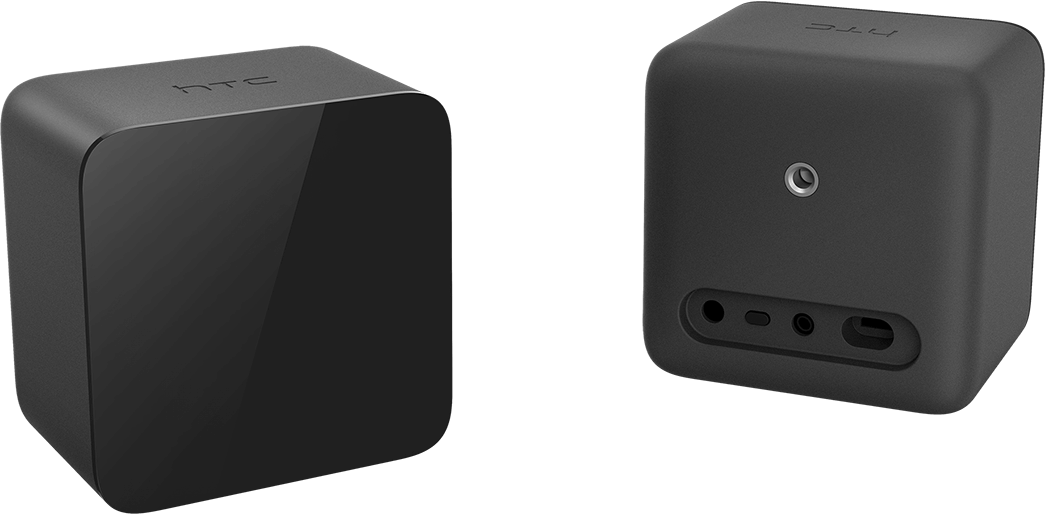
\includegraphics[width=0.6\textwidth]{img/base_stations.png}
\caption{The Vive Base Stations: laser-based tracking system (image source: \cite{VIVE}).}
\label{fig:BASE_STATIONS}
\end{figure}

\section{VR Sickness}

While VR is a promising technology, which quickly gains on popularity, it still has a great challenge and safety issue to overcome. Virtual reality sickness (also called cybersickness) is a group of unpleasant symptoms that can occur during an exposure to virtual environment. These symptoms can last from few minutes to even days. They most often include headache, disorientation, sweating, eye strain, fullness of stomach, pallor, vomiting, nausea, dryness of mouth, vertigo, or ataxia \cite{VRSYMPTOMSTIME}. Although similar to motion sickness, VR sickness is different in that it can occur with visual stimulation alone. Motion sickness is mainly induced with vestibular stimulation, while vision can be a contributing cause. It is also sufficiently different from simulator sickness that tends to occur as a result of oculomotor disturbances, with disorientation being the main symptom of VR sickness \cite{VRANDSIMULATORSICKNESS}. Beyond the sickness itself, these undesirable symptoms may have other consequences. VR sickness can reduce the efficiency of VR training and rehabilitation tools, and it can even discourage users from trying virtual reality ever again. Currently, there are many speculations as to why VR sickness occurs. J. J. LaViola in his article about cybersickness \cite{VRSYMPTOMS} describes three following main theories: 

\begin{itemize}
\item \textit{The sensory conflict theory}: The most commonly accepted theory. It is based on the assumption that inconsistency between the vestibular and visual sense cause a perceptual conflict within the body. These sensory conflicts may appear when the sensory input is not the stimulus that the user expected based on his prior experience. Taking this into consideration, the symptoms of VR sickness could be reduced if the sensory information causing self-motion are in agreement with each other.
\item \textit{The poison theory}: The theory tries to explain VR sickness from an evolutionary standpoint. It is based on the premise that the consumption of poison leads to physiological problems, temporarily affecting the coordination of sensory information. Nausea and vomiting serve as an early warning system that may increase the chances of survival. The conflicting stimulation found in VR can cause the misreading of sensory inputs, and it can make the body think that it has been poisoned.
\item \textit{The postural instability theory}: This theory focuses on the concept that the main objective of human body is to sustain postural stability at all times. If the control cannot be maintained, the motion sickness symptoms appear. In many virtual environments, there are some optically specified movements that are abnormal for inexperienced users. As a result, their postural control strategies may fail.
\end{itemize}

There are also other contributing factors to VR sickness, not necessarily related to any of these three theories. Various technical aspects can have a great impact on sickness symptoms, such as a mismatched motion, low refresh rate, or not achieving a target frame rate. Head position tracking is a vital element of any virtual environment, however, current tracking systems are not completely accurate. They can report information with error that leads to uncontrollable movement and dizziness. Studies have shown that increasing a field of view (FOV) tends to increase VR sickness symptoms. Implementing methods to dynamically restrict FOV can help combat this effect \cite{DYNAMICFOD}. Several other techniques are used to prevent VR sickness. For example, introducing static visual background (see Figure \ref{fig:STATIC_BACKGROUND}) allows users to register a verification of their senses while they observe the full locomotion of virtual environment. It has also been noted that some individuals are more susceptible than others to VR sickness \cite{VRINDIVIDUALS}. Age, health, postural stability, gender, experience with the system, and many other factors can contribute to the severity of the symptoms.

\begin{figure}[th]
\centering
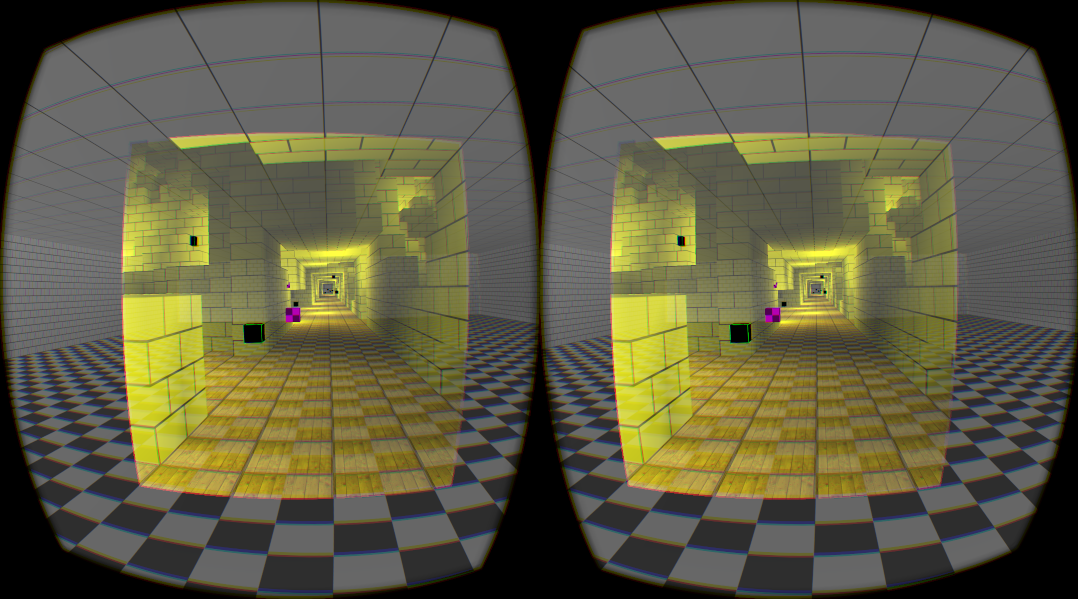
\includegraphics[width=0.85\textwidth]{img/static_background.png}
\caption{Static visual background, a technqiue used to reduce VR sickness symptoms (image source: \cite{STATICBACKGROUND}).}
\label{fig:STATIC_BACKGROUND}
\end{figure}

\section{Locomotion in VR}
Implementing locomotion in virtual reality is one of the biggest challenges of a creating comfortable and immersive VR experience. Poorly designed movement, such as sudden unexpected accelerations and rotations, can quickly induce sickness on even seasoned VR users. With the recent advancements in VR technology, numerous new locomotion techniques have been developed and researched \cite{VRHCI}. Unfortunately, there still has not been found the perfect approach that would work with equal efficacy across all users. Various methods have their strengths and weaknesses in terms of user experience, immersion, and input devices. 

In 2017, C. Boletsis published a systematic literature review \cite{LOCOMOTIONREVIEW} of recent studies investigating current VR locomotion techniques. In the 36 articles relevant to the research topic, he has identified the following 11 different methods of locomotion. 

\begin{itemize}
\item Arm swinging: The user stays in place and swings his arms. Body tracking devices or hand-worn controllers detect the arm movements that are then used to control VR locomotion.
\item Chair-based: This technique uses a stool chair as an input device. While sitting on it, the user can tilt and rotate the chair. These registered inputs are translated into VR forward, backward, and sideways motions.
\item Controller/joystick: The traditional input devices of video games. Using buttons for discrete input or joysticks for analog input, the user controls the movement in VR.
\item Gesture-based: Making hand gestures, such as push and tap, move the user in the virtual environment. Motion sensing input devices track the gestures that are translated into virtual movement.
\item Head-directed: The user controls locomotion with the help of equipped HMD. Yaw, pitch, or roll head motions command the direction and speed of VR movement.
\item Human joystick: This method uses a sensing board (e.g., Wii Balance Board). By leaning on it, the user can produce the backward, forward, and sideways motions.
\item Real-walking: While the user moves freely within a limited physical space, body tracking devices are used to determine his position in the virtual environment.
\item Redirected walking: The user explores a virtual world that is significantly larger than the limited physical space. This approach introduces a subtle mismatch between virtual and real movements to wrap the enormous virtual environment into the tracked physical space.
\item Reorientation: As in the case of the redirected walking, the user physically walks without restrictions while exploring the unlimited virtual world. This technique modifies the rotational gain of the user. The modification forces him to unknowingly reorient himself when he meets the boundaries of the physical space.
\item Teleportation: By making a pointing gesture or using a controller, the user indicates where he wants to move in the scene. He is then immediately teleported to the new location he has just pointed with the controller.
\item Walking-in-place: The user makes a walking motion. Input is registered with motion trackers or with the help of treadmill-like navigation devices.
\end{itemize}

In his literature review, C. Boletsis proposes locomotion typology with four different classification categories (see Figure \ref{fig:TYPOLOGY}). The first of them is an interaction type. It focuses on the methods of triggering VR navigation. Artificial methods utilize various input devices, while physical methods exploit motion cues with body tracking devices. Next category, a VR motion type, separates techniques into continues and non-continues motions. Continues motion offers a smooth, uninterrupted movement, whereas non-continues motion provides instantaneous teleport transitions. A VR interaction space is the third classification category. It can be limited due to the constraints of the physical environment, or it can be open and support the unlimited movement in the virtual environment. Lastly, the techniques can be classified into four distinct VR locomotion types:

\begin{itemize}
\item Motion-based: These locomotion techniques support the continuous movement in open interaction space with some kind of physical motions. This type includes methods such as the arm swinging, gesture-based, redirected walking, reorientation, and walking-in-place locomotion.
\item Room scale-based: The techniques that support continuous movement and utilize interaction with physical movement. However, as opposed to motion-based methods, the interaction space is limited by the physical environment's size. From the previously mentioned techniques, only the real-walking locomotion matches this description.
\item Controller-based: The methods under this type use various controllers for continues movement in open interaction spaces. Locomotion techniques such as the human joystick, chair-based, head-directed, and joystick-based fall under this type.
\item Teleportation-based: This locomotion type uses artificial interactions in open interaction spaces. It differs from the controller-based methods in the non-continues movement, as the user is immediately teleported to the selected position. This type includes the free and fixpoint teleport techniques.
\end{itemize}

\begin{figure}[th]
\centering
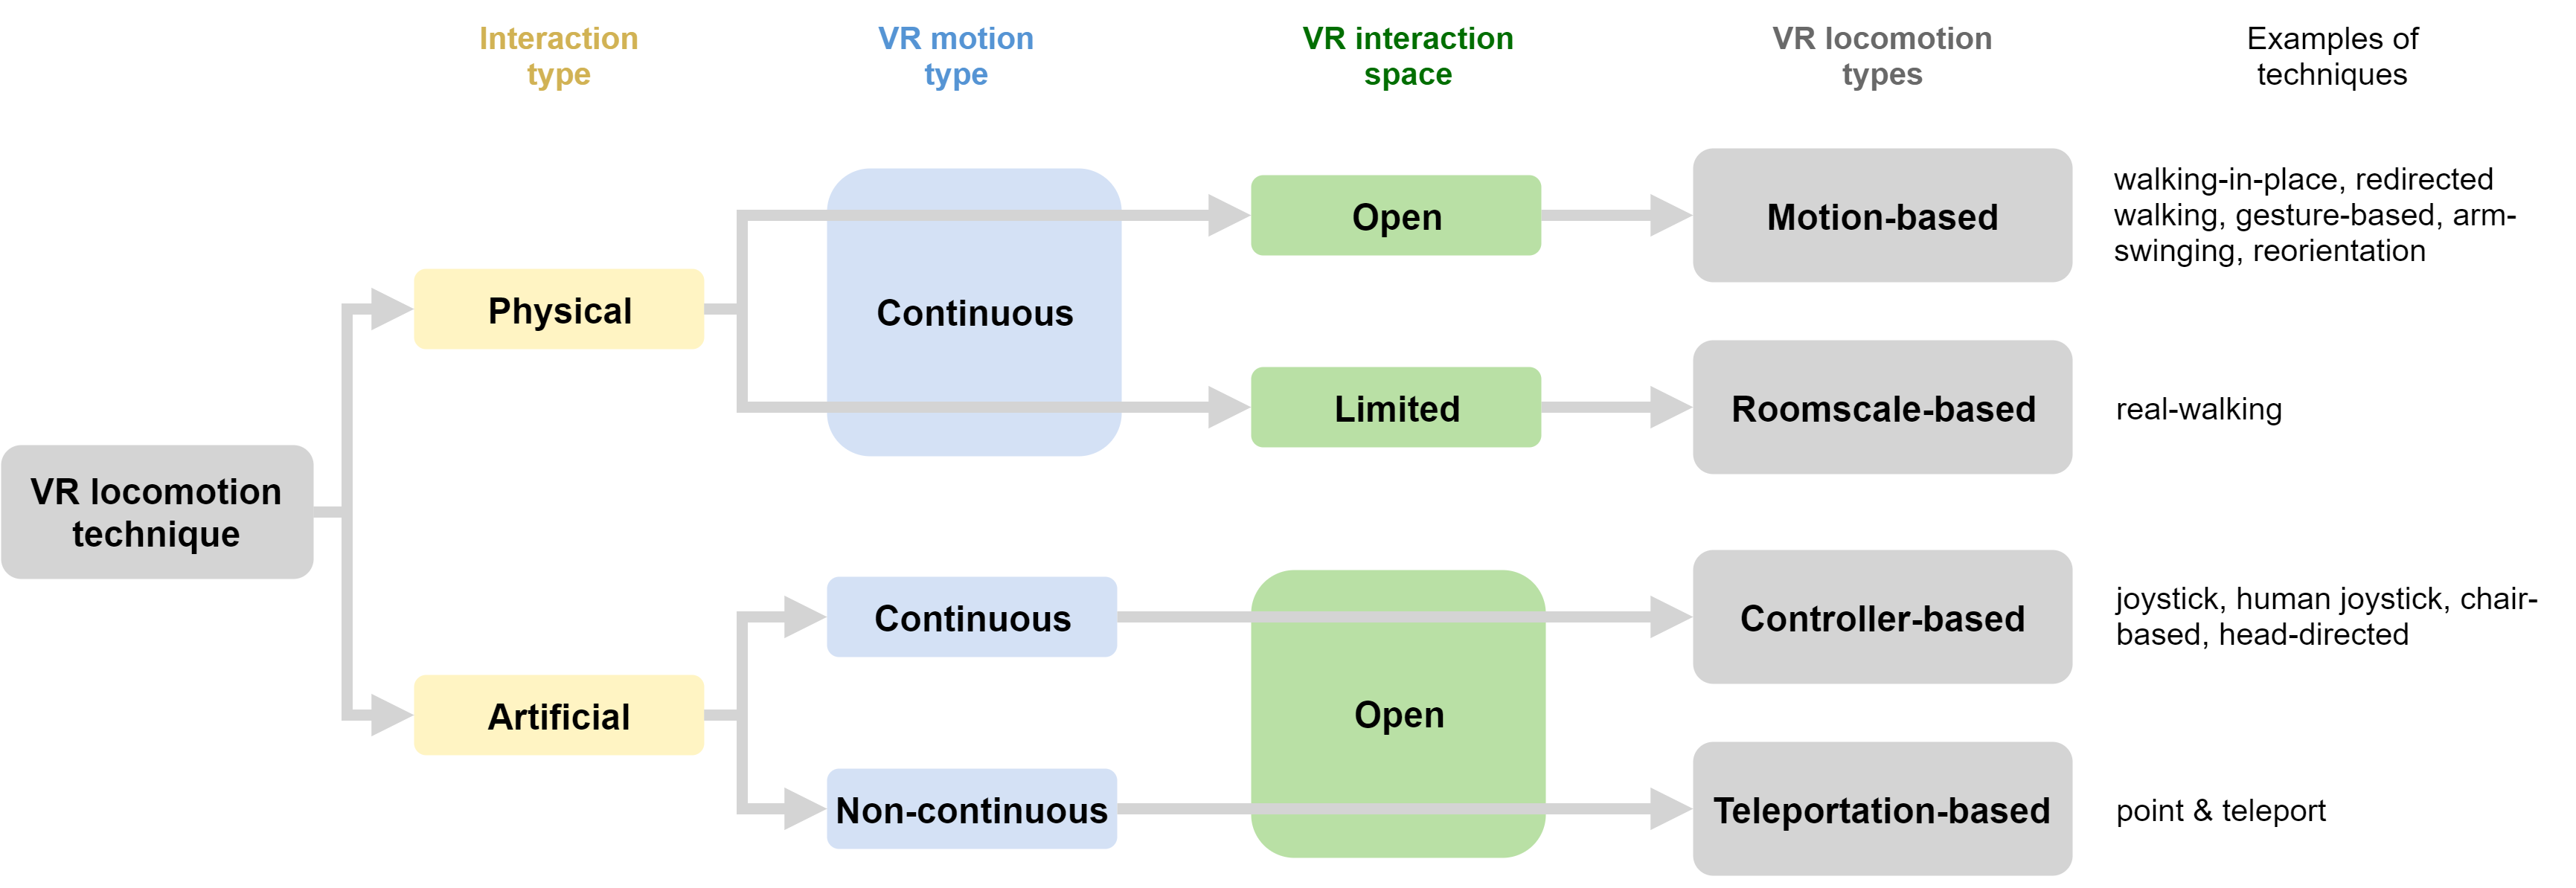
\includegraphics[width=1\textwidth]{img/locomotion_typology.png}
\caption{The VR locomotion typology (image source: \cite{LOCOMOTIONREVIEW}).}
\label{fig:TYPOLOGY}
\end{figure}

Although there are many promising solutions to VR locomotion, currently only a handful of them are used in mainstream VR games. Approaches like the real-walking, reorientation, or redirected-walking locomotion offer creative way of exploring the virtual world, however, they often require a dedicated and expensive hardware, large tracking space, and can be tiring in longer VR sessions. For these reasons VR developers mostly implement regular controller-based locomotion techniques. Unfortunately, the joystick-based continuous motion is known for inducing VR sickness symptoms. This problem is now partly solved with effective dynamic field-of-view adjustments \cite{DYNAMICFOD}. Many popular VR games, such as Robo Recall, Raw Data, and Vanishing Realms, adopt the Point \& Teleport locomotion to reduce the effects of motion sickness \cite{TELEPORTATIONGAMES}. This technique uses a pointing curve as the indicator for the teleportation path (see Figure \ref{fig:TELEPORTATIONCURVEIMAGE}). Although it has been proved by some researchers to be the least discomforting locomotion method for the VR users, its drawback is that it can also reduce a sense of presence within the VR environment \cite{TELEPORTATIONEFFECTS}. An alternative fixpoint teleport locomotion, which allows the player to quickly move between predefined node positions, can be applied to preserve accessibility while maintaining the feeling of presence \cite{NODEBASEDTELEPORTATION}.

\begin{figure}[th]
\centering
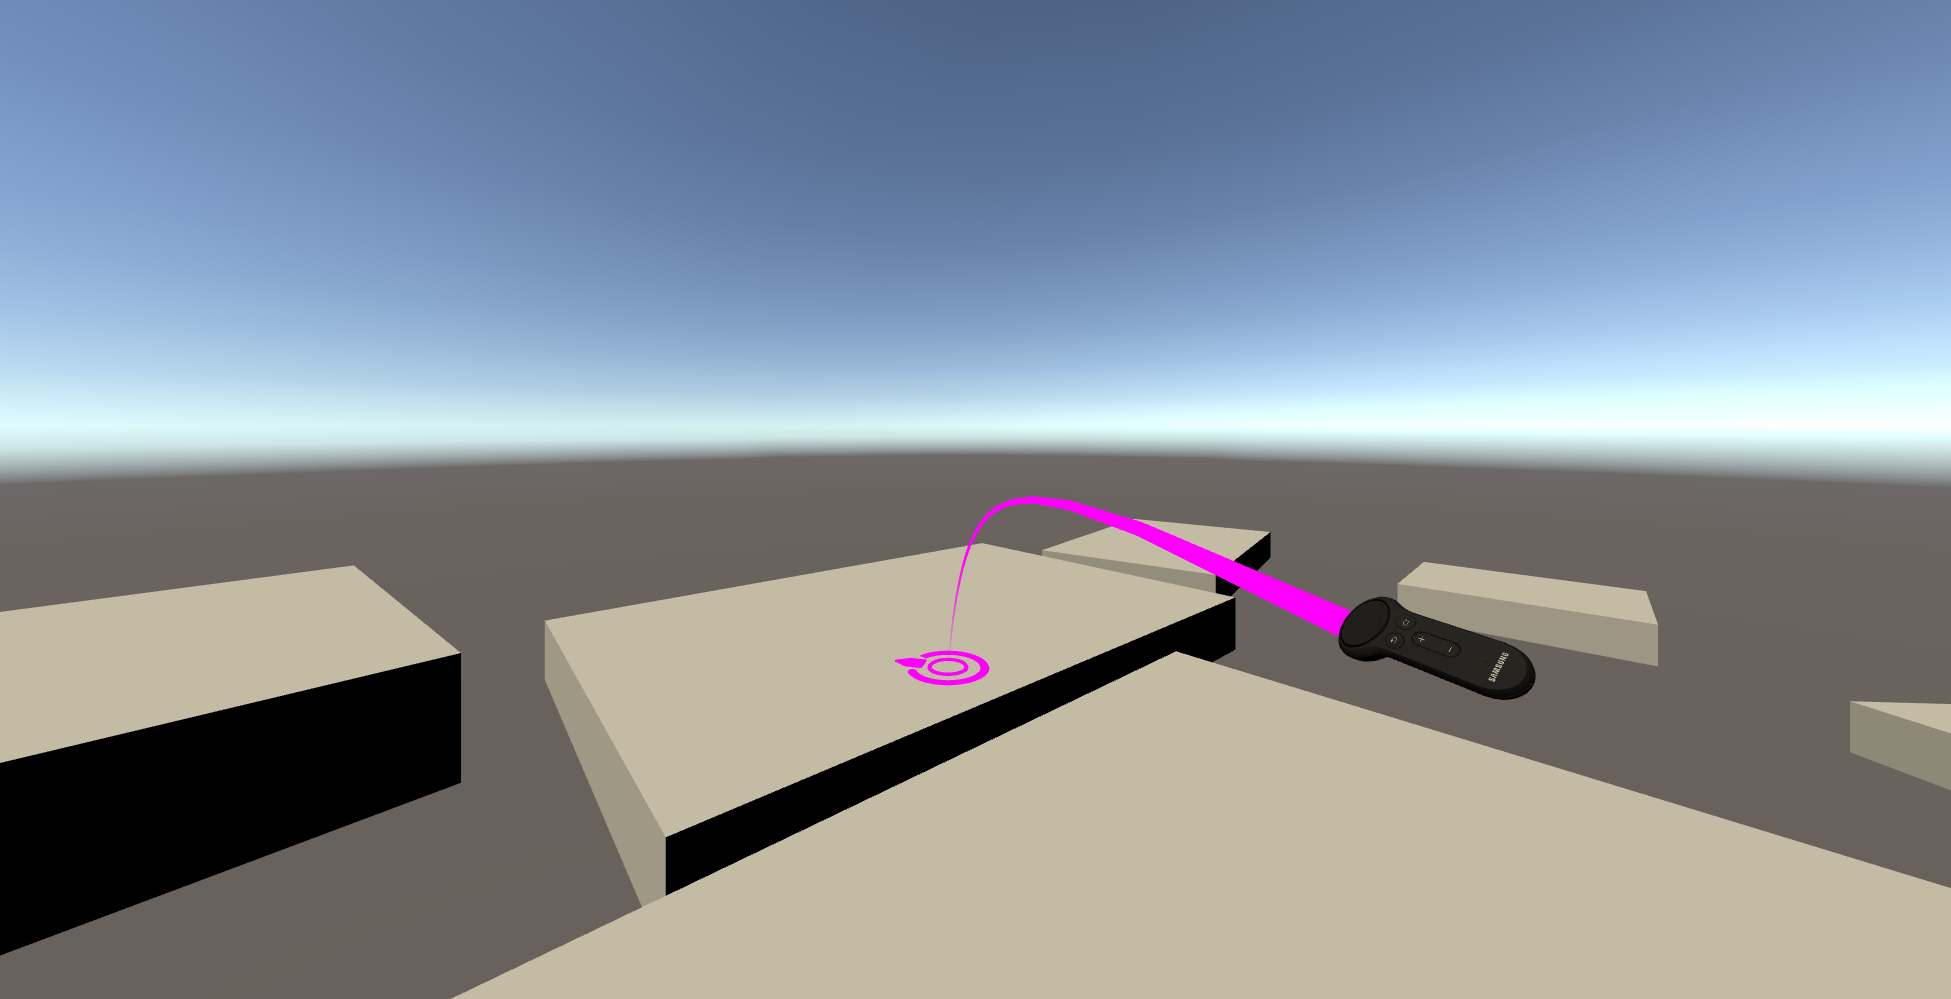
\includegraphics[width=0.77\textwidth]{img/teleportation_curve.png}
\caption{The Point \& Teleport locomotion technique that uses a curve as the indicator for the teleportation path (image source: \cite{TELEPORTATIONCURVE}).}
\label{fig:TELEPORTATIONCURVEIMAGE}
\end{figure}

There are several tricks and best practices for designing VR locomotion. Oculus in their developer documentation \cite{OCULUSDOC} lists general guidelines for acceleration, speed, user control, and direction of locomotion. Accelerations in VR not initiated by the user's physical movement are the main cause of discomfort. It is best to avoid any unpredictable increases of the size, frequency, and duration of the acceleration. Manipulations of speed, such as a slow-motion or unnaturally rapid velocity, have been reported to be less discomforting than a normal human pace. In the real world, humans most often move forward or stand in place. When the VR movement is necessary, it is best to prevent backing up or strafing movements as it can be unusual optic flow pattern to the users. Open environments are also generally more comfortable. Moving the users through enclosed spaces, such as tunnels or hallways, should be avoided.

\section{Problem of VR Head Collisions}

Although modern VR games use different techniques to move the player's avatar in the virtual environment, most of them have one thing in common. They use tracking systems to estimate the position and rotation of the user's head. The player now gets the ability to look around the virtual world with physical head movements without the need of additional input controllers. Head tracking increases the feeling of presence in virtual reality. It also drastically reduces VR sickness symptoms that are caused due to the mismatch between vestibular and visual senses \cite{HEADTRACKINGSYMPTOMS}. However, positional head tracking introduces a significant problem with head-object collisions in the virtual scene.

In traditional video games, a virtual camera used to render a game world is under full control of the game logic. It usually follows the player's avatar in a first-person or third-person view, or it is set during the game creation to some fixed position and orientation. The game engine then renders an image of the virtual world for that camera setup. For the most part, video games use collision detection systems to prevent the intersection of two or more objects on the game scene. If the player collides with some game object, such as a table or wall, the player's avatar and the camera stop moving in that direction. The user is under the impression that he has been physically blocked by the object. 

With the addition of head tracking to VR games, some of the camera control rules change or become obsolete. Almost all VR games are playable only in the first-person view. This makes the players feel immersed and present in the virtual world. The camera's position still follows the avatar's head, but the camera's rotation is now set using the player’s real-world head rotation. Unfortunately, head tracking also changes the way how head-object collisions are normally resolved in games. The problem arises when the player's head should collide with some game object, but the user keeps moving his head in real-world without any obstructions. There are researchers that experiment with a haptic system that can simulate walls or heavy objects via electrical muscle stimulation \cite{HEPTICSYSTEM}. However, it could take years before this technology works properly and becomes available to the mainstream VR users. With the recent popularity of VR games, there is a need for solution that could be adapted by current VR developers.

\begin{figure}[th]
\centering
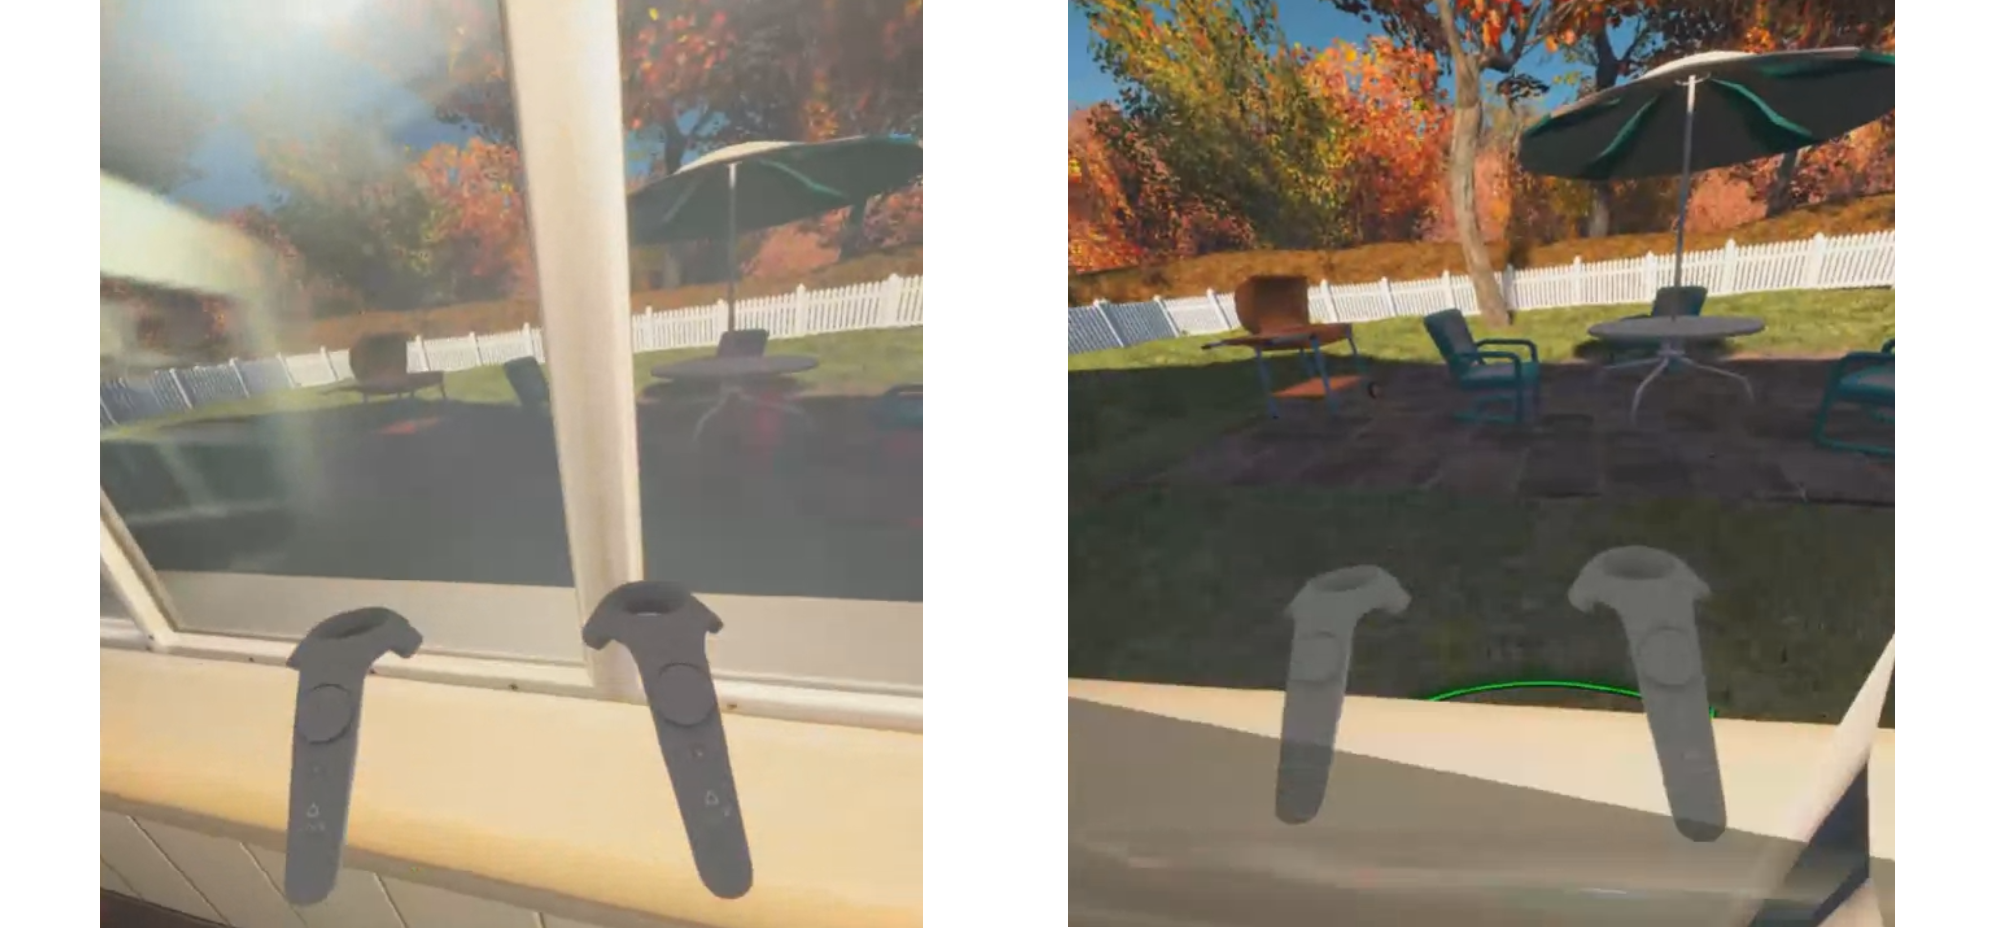
\includegraphics[width=1\textwidth]{img/clipping.png}
\caption{In the game Fallout 4 VR, players can see through walls when they lean against them (image source: \cite{redditfallout}).}
\label{fig:FALLOUTCLIPPING}
\end{figure}

Many developers ignore the problem of head collisions and decide to not handle it in any way \cite{OCULUSDOCCLIPPING}. If the player positions himself close to some obstructing object in the virtual scene and then starts leaning in the direction of the collision, the head rotation will still update according to the real-world position. The player will be able to look inside or past the colliding object. This results in unexpected clipping artifacts (see Figure \ref{fig:FALLOUTCLIPPING}) that break the feeling of presence in virtual world. The ability to see through the game objects can also have undesirable effects on game mechanics. In games with the Point \& Teleport locomotion, the players can cheat by teleporting through walls to skip harder game areas \cite{SKYRIMTELEPORT}. In shooter games, the players can see and shoot through walls, giving them an unfair advantage over enemies. There is a need for solution that would at least restrict the forbidden view. For these reasons, many VR developers try various techniques for handling head collisions in their games. The most commonly used methods are:

\begin{itemize}
\item Screen fade: When the head collision is detected, the screen slowly fades to black or any other solid color (see Figure \ref{fig:SCREENFADEIMAGE}). The view remains blacked-out for as long as the player's head collides with the object. Because this technique is relatively simple to implement, it attracts many VR developers looking for a quick solution to the problem. However, the method has one weakness that makes it not work well with the Point \& Teleport locomotion technique. For example, the player can unintentionally teleport to some head-object colliding position. He is then stuck in a black void, without knowing in what direction he should move his head to escape the darkness.

\item Delayed push-back: If the player collides with some object for a couple of seconds, he is gradually pushed backwards until he leaves the object's boundaries. This method is often used in older open-world games that were nowadays ported to VR, such as Skyrim VR or Fallout 4 VR. In most implementations of this technique, the head tracking is completely disabled during the duration of the push-back effect. Many players of these games reported that the camera push-back is frustrating to experience and makes them feel dizzy \cite{redditfallout}\cite{SKYRIMVRPUSHBACK}\cite{PUSHBACKFEEDBACK}. The reason is that the push-back effect takes control of camera movements away from the player, which tends to increase VR sickness symptoms.

\item Instant push-back: In this solution, the collisions are handled similarly to how they are handled in most non-VR games; the player's virtual body, including the head, is never able to get past virtual walls and other obstacles. When the user collides with some obstacle, a collision vector is computed and its projection on the horizontal plane is added to the player's position. This effectively moves the user away from the object, preventing him from ever looking inside it. If the player decides to keep moving his head forward, despite the fact that there is a virtual wall in front of him, he will feel like he is using his head to push himself backwards from the wall. In 2018, a group of researchers \cite{COMPARISONCOLLISION} experimented with this technique, which they called a ``not there yet'' approach. The researchers compared this solution to the screen fade method in terms of immersion and VR sickness. Unfortunately, they found out that while the ``not there yet'' approach yielded better immersion results, it contributed more to VR sickness symptoms.

\item Teleportation: If the collision is detected and maintained for a couple of seconds, the player is teleported to a nearby collision-free location. This method works similarly to delayed push-back, but instead of gradually moving the player away from the obstacle, he is instantly teleported to the last know valid position. Virtual Reality Toolkit, a collection of useful concepts and scripts that aid building VR applications, offers an implementation of this method that can be adjusted by many parameters \cite{VRTK_REWIND}. For example, developers can set the amount of time for the teleportation delay or the additional push-back distance, which prevents the player from being right next to the obstacle again after the teleportation occurs. 
\end{itemize}

\begin{figure}[th]
\centering
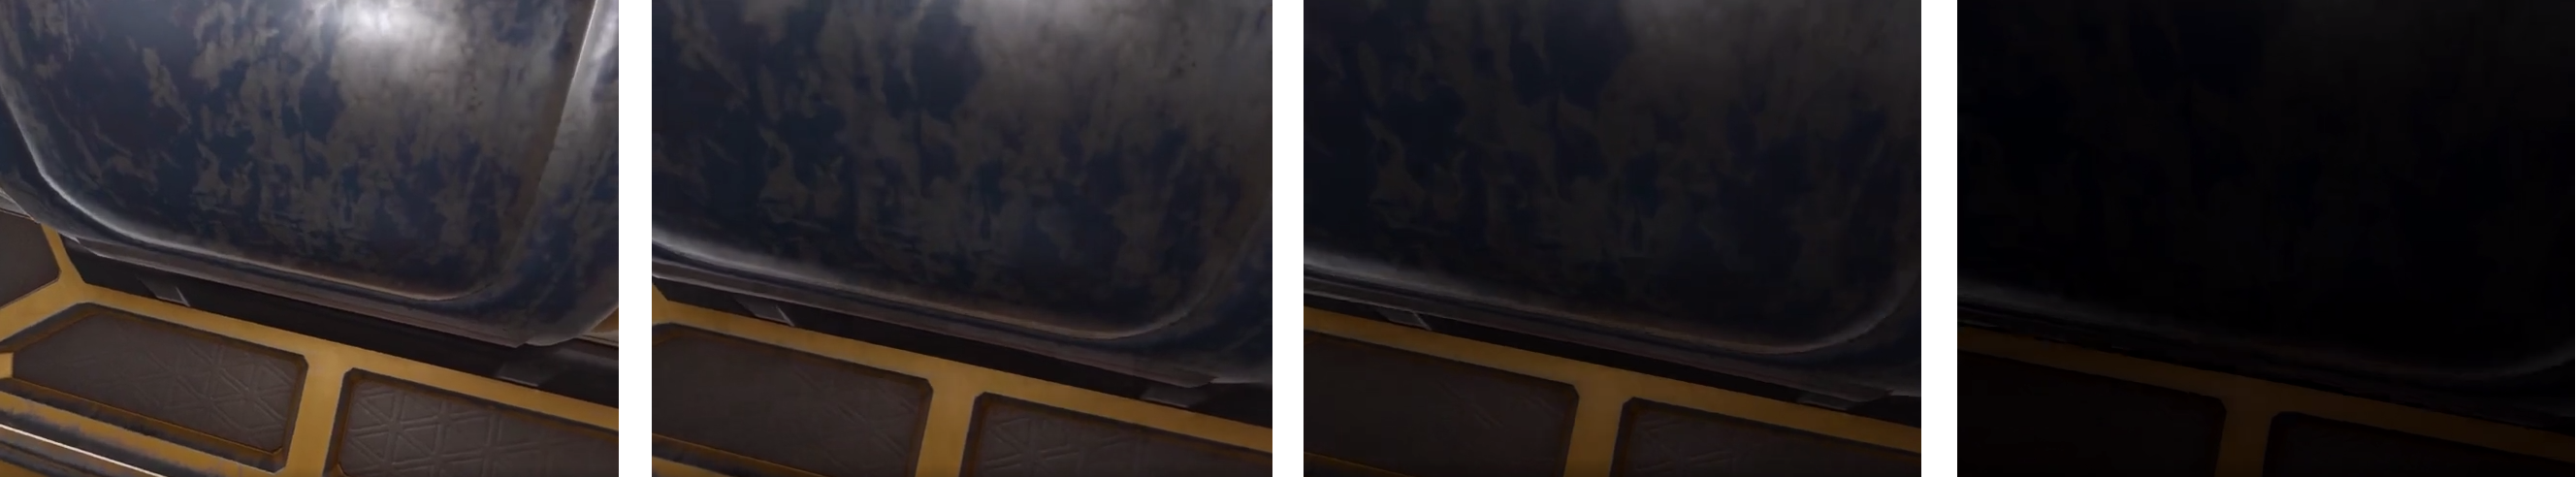
\includegraphics[width=1\textwidth]{img/screen_fade.png}
\caption{A time slice example of the screen fade technique. When the head collision is detected, the screen slowly fades to black (image source: \cite{SCREENFADE}).}
\label{fig:SCREENFADEIMAGE}
\end{figure}

\begin{figure}[th]
\centering
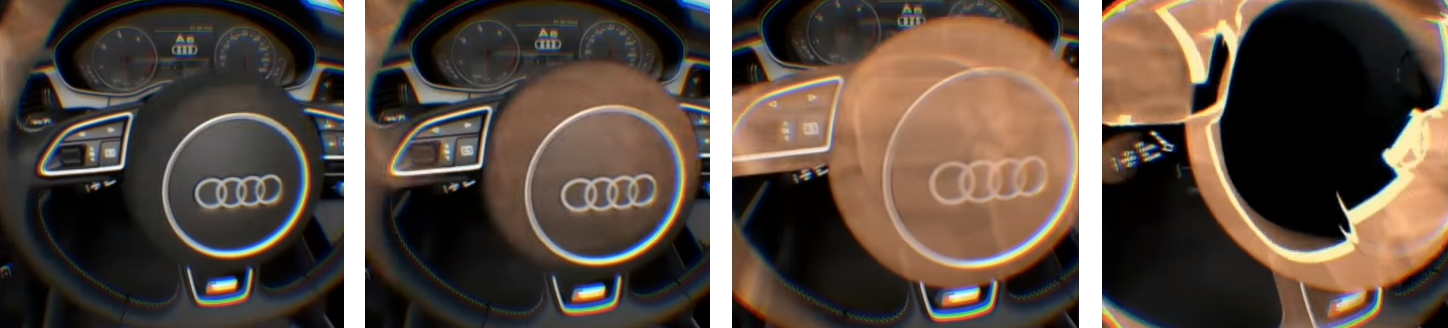
\includegraphics[width=1\textwidth]{img/object_fade.png}
\caption{A time slice example of the object fade technique. The closer the camera gets to the collision, the more the colliding object is faded out (image source: \cite{OBJECTFADE}).}
\label{fig:OBJECTFADEIMAGE}
\end{figure}

Sometimes the solutions mentioned above are slightly modified to fit the aesthetic of the game. For instance, the solid color in the screen fade technique can be replaced by any image or virtual scene. There are also some other, less popular ideas for solving the head collisions problem. Object fade is a technique in which, rather than fading the whole screen to black, only parts of the colliding objects fade out as the camera gets closer to them (see Figure \ref{fig:OBJECTFADEIMAGE}). The advantage of this solution is that the player can easily recognize which specific objects are colliding with him. If he unintentionally teleports to some head-object colliding position, he can maneuver his head out of the highlighted objects. He can also completely avoid any collisions by tracking the color of surrounding obstacles. If some object starts to fade, the player knows to not get any closer to it. 

Some VR developers try completely different approach by designing the whole gameplay around collisions. The virtual environment is carefully designed in the way that prevents the players from colliding with any object in the game. The problematic collisions are then avoided all together by restricting the movement to only specific game areas. In other VR games, the collisions are the main objective of the gameplay. The central mechanic is to collect or destroy some objects that disappear when they collide with the player, making it impossible to look inside them \cite{ELEVR}. 

\section{Conclusion}

In recent years, there has been growing interest in VR technology. Modern VR headsets offer an affordable VR experience that is easy to set up in a home setting. The HTC Vive aims at providing immersive room-scale VR, whereas other companies focus on seated experience that does not require a large tracking space and additional inside-out tracking devices. The hand worn controllers, which support 6DoF tracking information, are the current standard for handling input in almost every VR system. They track the movement of the user's hands, allow him to pick up objects in the virtual world, and are useful in many locomotion techniques. In the Point \& Teleport technique, they allow for an easy manipulation of the teleportation curve. Most often, VR headsets are also equipped with some sort of the head tracking system. Head tracking greatly increases the feeling of presence in virtual world and reduces the symptoms of VR sickness.

The commercial success of VR headsets has brought the attention of many academic researchers. There have been a lot of studies into comfortable and immersive locomotion techniques that can be used in virtual reality. VR experience is often measured using questionnaires about the satisfaction of being in VR, the sense of presence in VR, and the symptoms of simulator sickness. The consensus is that the teleportation methods are best suited for the seated VR experience in terms of usability and preventing VR sickness. Although the topic of locomotion is widely studied, researchers have not treated head tracking in much detail. Apart from the recent study about ``not there yet'' approach, there is almost no academic work on the problem of VR head collisions. This thesis examines the most popular methods for solving the problem and tries to propose the best solution.